% Section VI: Single-Condition System Behaviour. Characterises C1 (operational
% LCP-WS-L1) in isolation before the comparative analysis. Five subsections.
% Prose ported and adapted from References/Artifact_discussions.md §VI.

We first characterise the operational behaviour of the LCP-WS-$L_1$ planner ($C_1$ in Table~\ref{tab:conditions}) in isolation, before introducing the WS-vs-cascade comparison of Section~\ref{sec:results}. The aim is to establish the qualitative and quantitative envelope of the operational planner on the 16-scenario benchmark: which rules fire on which scenarios, what the typical violation magnitudes look like, and what the per-tick visualisation reveals about the planner's micro-behaviour.

\subsection{The Benchmark}
\label{sec:singlecondition:benchmark}

Table~\ref{tab:per_scenario_status} (auto-generated; presented in Section~\ref{sec:results:compromise}) reports the per-scenario outcomes of the LCP-WS-$L_1$ sweep on the 16-scenario benchmark under $C_1$ (seed $= 7$). The planner completes every scenario; the top-violating MPC-controlled rule lives at $L_7$ on 11 of 16 scenarios (\texttt{7r2} Opposing Lane on 10 scenarios, \texttt{7r1} Traffic Light on 1), at $L_3$ on 4 scenarios (\texttt{3r3} Safe Headway, \texttt{3r0} Speed Limit, \texttt{3r5} Lateral Clearance), and at $L_0$ on 1 scenario (\texttt{0r3} Lateral Comfort). We use the table as orientation for the per-tick and per-level views that follow.

\subsection{Per-Scenario Visualisation}
\label{sec:singlecondition:viz}

\begin{figure}[t]
    \centering
    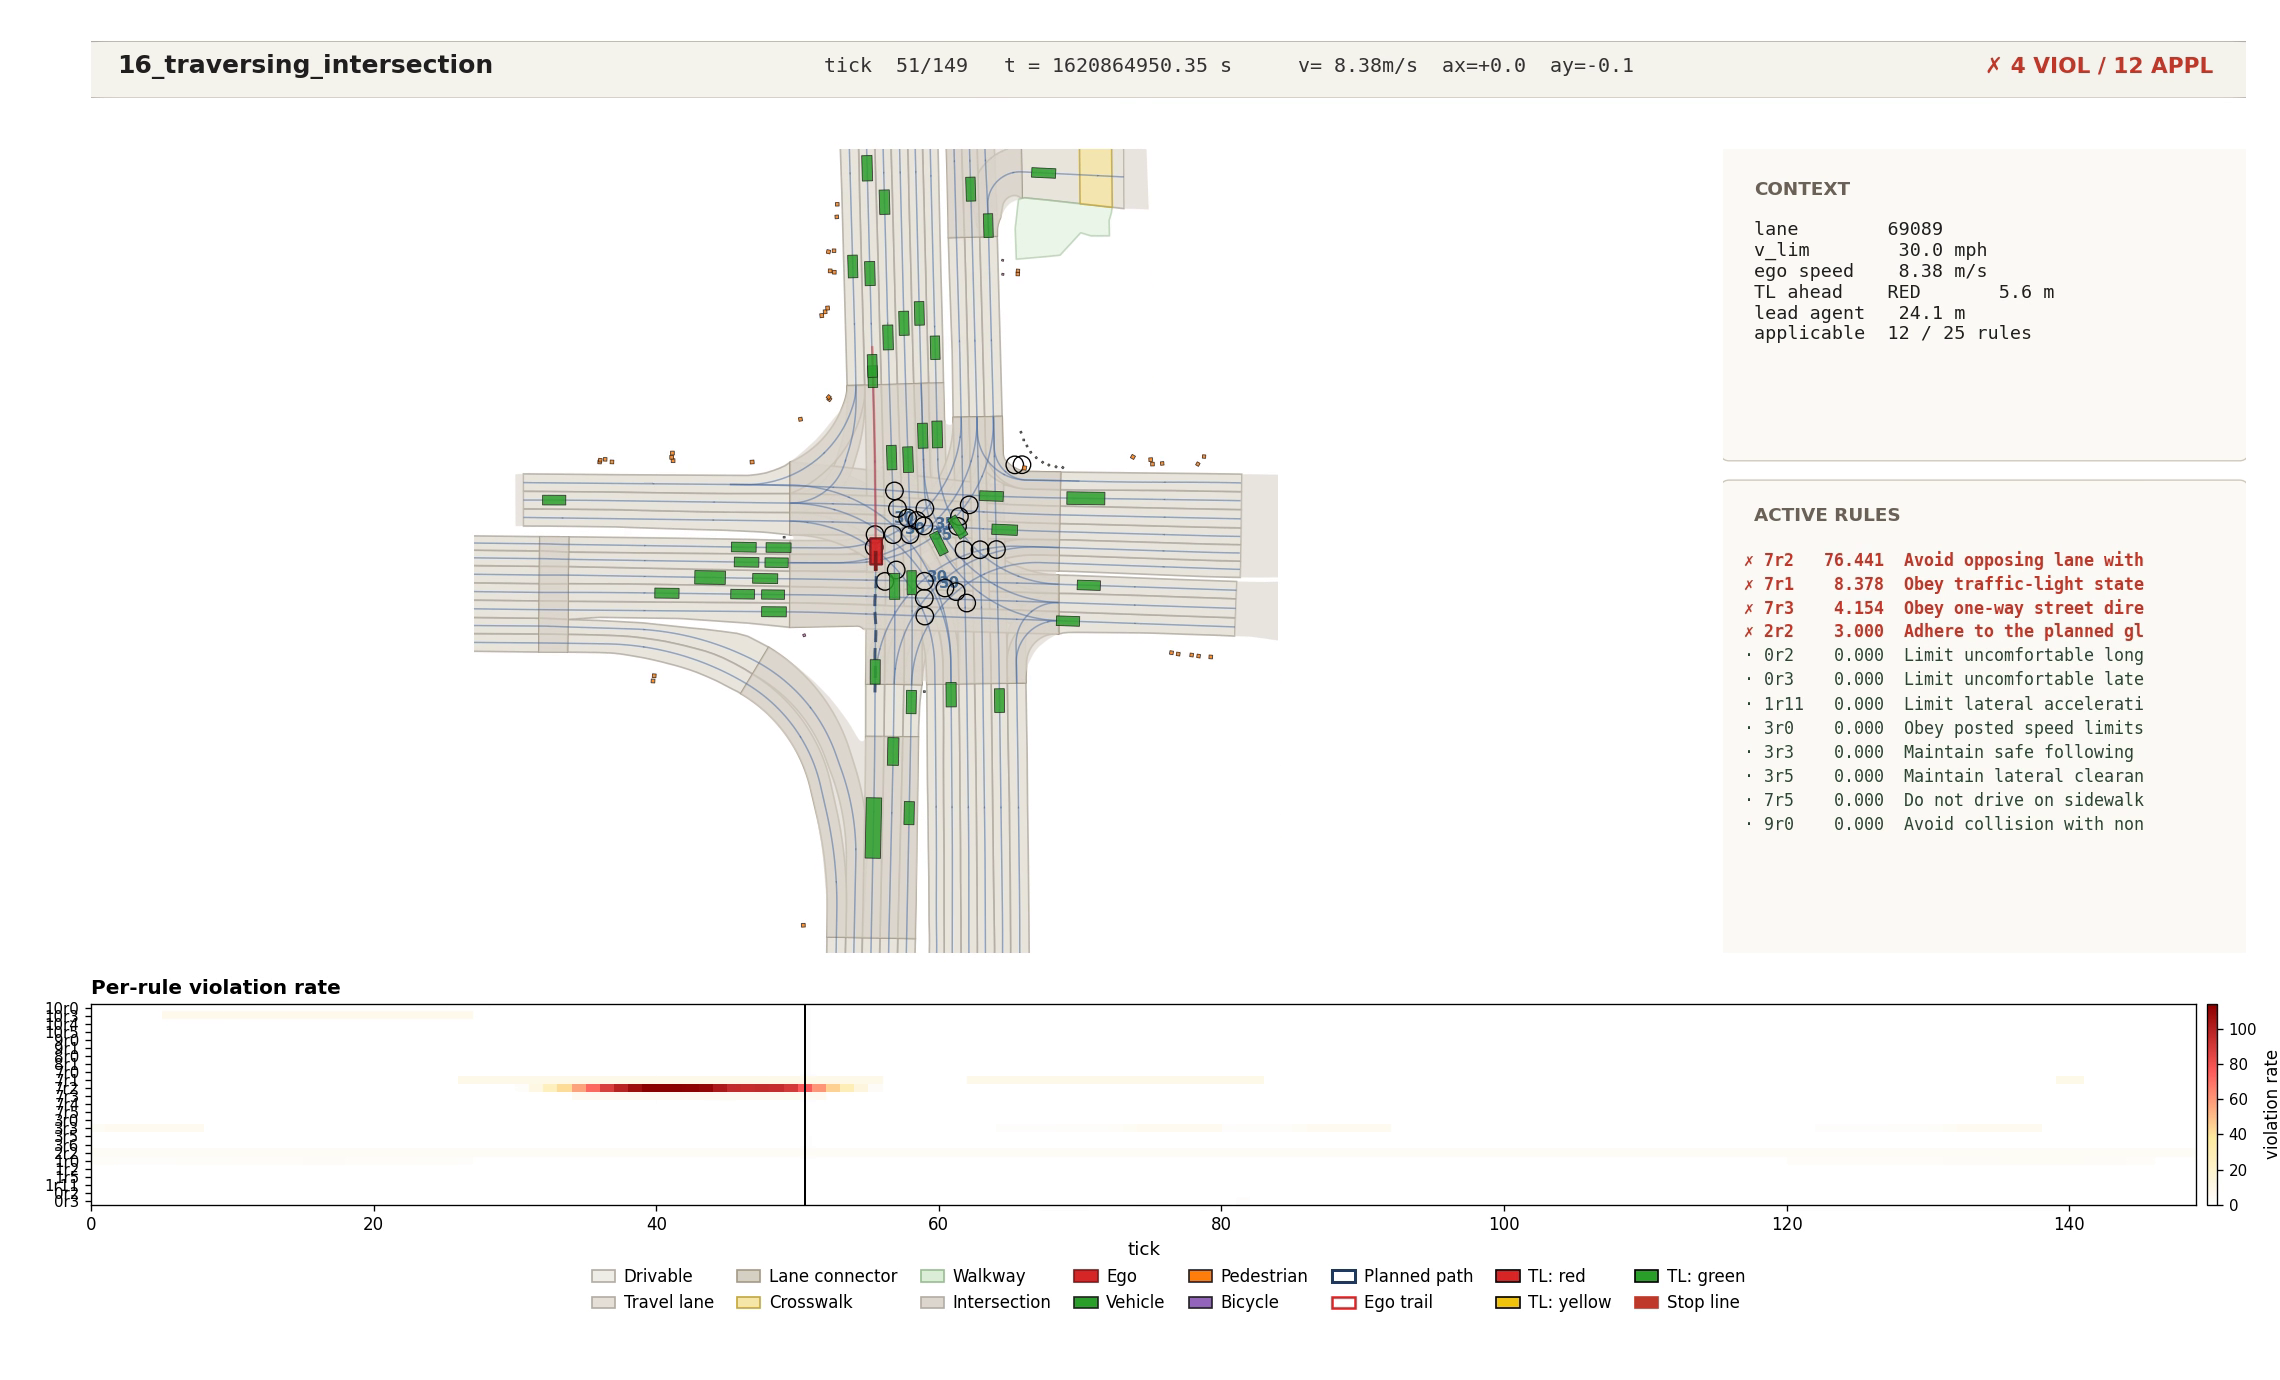
\includegraphics[width=\linewidth]{./Figures/fig09_qual_frame}
    \caption{Single frame from the LCP-WS-$L_1$ traversal of \texttt{16\_traversing\_intersection}. The visualisation places the ego (red) in the lane geometry with the planned trajectory (dashed). The right-hand sidebar shows the active rules sorted by violation rate at the displayed tick; the bottom strip shows the per-rule violation rate over the full episode with the displayed tick marked. The full 16-scenario \texttt{.mp4}/\texttt{.gif} gallery + per-scenario READMEs are in the online supplementary material.}
    \label{fig:qualitative_frame}
\end{figure}

Fig.~\ref{fig:qualitative_frame} shows a representative single frame from the per-tick visualisation, selected from the scenario at which the planner traverses a complete signalised intersection. We use the visualisation throughout the deployment phase as the qualitative complement to the per-tick rule-evaluation logs: discrepancies between the expected and the observed behaviour on a particular tick are first investigated by locating the corresponding frame, after which the per-tick CSV is inspected for the relevant rule's applicability and violation flags. The visualisation honours the design rule that no text element overlays the map area; lane-id labels are restricted to the ego's immediate neighbourhood (radius $14$~m) and show only the speed limit in small, subtle text.

\subsection{Cross-Scenario Aggregate Patterns}
\label{sec:singlecondition:aggregate}

\begin{figure}[t]
    \centering
    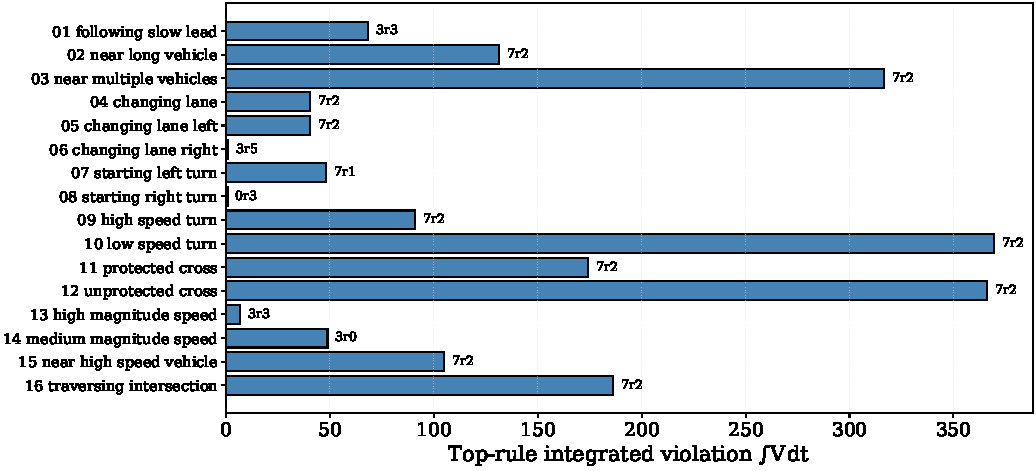
\includegraphics[width=\linewidth]{./Figures/fig10_top_violation}
    \caption{Per-scenario top-rule integrated violation under condition $C_1$, restricted to the 13 MPC-controlled rules of Section~\ref{sec:rulebook:partition}. The distribution is dominated by intersection, lane-change, and turn scenarios at $L_7$ (legal: opposing-lane and traffic-light constraints, 11 of 16 scenarios) and by speed/headway scenarios at $L_3$ (4 of 16); one scenario tops at $L_0$ lateral comfort.}
    \label{fig:a1_top_rule}
\end{figure}

\begin{figure}[t]
    \centering
    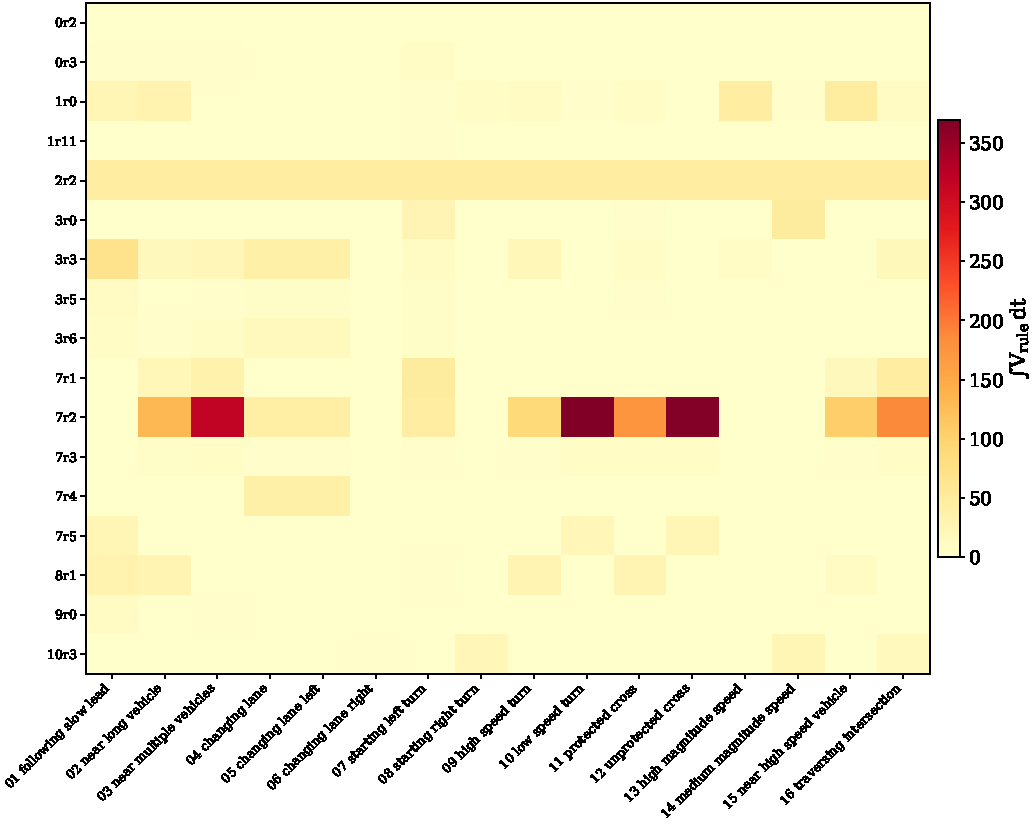
\includegraphics[width=\linewidth]{./Figures/fig11_rule_scenario_heatmap}
    \caption{Per-rule per-scenario integrated-violation heatmap under condition $C_1$. Rows are the union of MPC-controlled and observer-only rules of Table~\ref{tab:rulebook} that record any non-zero integrated violation on any benchmark scenario; columns are the 16 benchmark scenarios; rows are sorted by descending priority level. The cell colour encodes $\int r(t)\,\mathrm{d}t$ over the rule's applicable ticks. The block structure is a useful empirical fingerprint: turn and intersection scenarios share a common MPC-rule signature (\texttt{7r1}, \texttt{7r2}, \texttt{7r5}); lane-change scenarios additionally trigger the observer-only \texttt{2r2} (Route Adherence); high-density following scenarios are bound by the comfort and headway rules (\texttt{3r0}, \texttt{3r3}).}
    \label{fig:a3_rule_x_scenario}
\end{figure}

\begin{figure}[t]
    \centering
    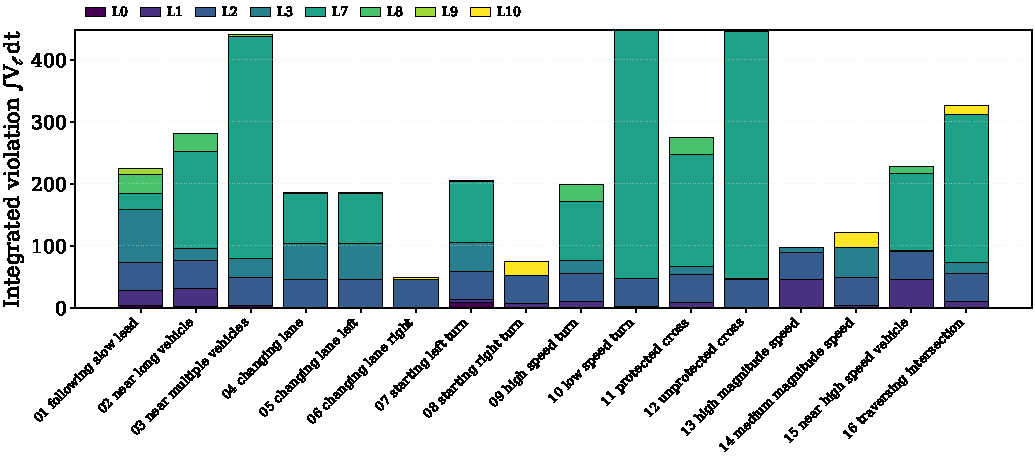
\includegraphics[width=\linewidth]{./Figures/fig12_level_breakdown}
    \caption{Per-scenario stacked integrated violation under $C_1$, broken down by priority level. Each bar is a scenario; each stacked segment is a priority level. The figure establishes the per-level violation vector $V_{\mathrm{MPC}, \ell}$ of Definition~\ref{def:per-level-violation} --- the primary structural metric of Section~\ref{sec:results} --- at a glance.}
    \label{fig:a5_level_breakdown}
\end{figure}

Fig.~\ref{fig:a1_top_rule} reveals the per-scenario distribution of the dominant MPC-controlled violation under the operational condition $C_1$. The dominant rule tracks the scenario semantics: turn, intersection, and lane-change scenarios are bound by \texttt{7r2} (Opposing Lane) and \texttt{7r1} (Traffic Light) at $L_7$; high-density following scenarios are bound by \texttt{3r3} (Safe Headway) and \texttt{3r0} (Speed Limit) at $L_3$; one sharp-right-turn scenario is bound by \texttt{0r3} (Lateral Comfort) at $L_0$. We use this distribution to motivate the per-level analysis in Section~\ref{sec:results}.

Fig.~\ref{fig:a3_rule_x_scenario} provides the rule-by-scenario decomposition of the integrated violations under $C_1$. The block structure of the heatmap is a useful empirical fingerprint of the rulebook: turn and intersection scenarios share a common rule signature distinct from the lane-change signature; the high-speed scenarios isolate the comfort and headway rules (\texttt{3r0}, \texttt{3r3}). The figure motivates the scenario-class keying used by the calibration cache (Section~\ref{sec:deployment:cache}): the cache stores one $(w^{\dagger}, b_{\epsilon}^{\star})$ pair per scenario class because the active rule set is approximately constant within a class and changes between classes.

Fig.~\ref{fig:a5_level_breakdown} complements Fig.~\ref{fig:a3_rule_x_scenario} by aggregating along the rule dimension up to the priority level. We observe that the violation mass is concentrated at $L_7$ (legal) in intersection, turn, and lane-change scenarios; at $L_3$ (speed and headway) in high-density following scenarios; and that the high-priority collision-avoidance levels $L_{10}$ and $L_9$ are zero on every scenario --- the planner holds them effectively hard, consistent with the benign-but-nontrivial nature of the \texttt{nuPlan-mini} benchmark. The figure establishes the per-level violation vector $V_{\mathrm{MPC}, \ell}$ of Definition~\ref{def:per-level-violation} at a glance.

The remaining cross-scenario aggregate figures are released as online supplementary material. Briefly: \texttt{A2} (per-rule aggregate violation) sums each MPC-controlled rule's integrated violation across the 16 scenarios, revealing which rules dominate the benchmark's overall violation mass; \texttt{A4} (per-rule violation-tick count) counts the number of ticks at which each rule is violated, complementing \texttt{A2} by separating short high-rate bursts from sustained low-rate violations; \texttt{A6} (applicability frequency) reports per-rule applicability rate, useful for identifying which rules govern the largest time windows of the benchmark; \texttt{A7} (rule-co-occurrence matrix) is a $25 \times 25$ matrix whose entry $(i, j)$ counts ticks at which rules $i$ and $j$ are simultaneously violated, exposing rule-interaction patterns; \texttt{A8} (burst-duration distribution) reports per-rule the distribution of consecutive-tick violation runs, separating ``always-on'' rules from intermittent-burst rules; \texttt{A9} (four-panel dashboard) is a composite of the most-watched aggregates; \texttt{A10} (scenario-similarity dendrogram) clusters the 16 scenarios by cosine similarity of their per-rule violation profiles, revealing the natural scenario-class structure that motivates the calibration-cache keying.

\subsection{Per-Scenario Detail}
\label{sec:singlecondition:detail}

The per-tick observer log emitted by the batch driver is the primary forensic artefact at single-scenario resolution. For any scenario in Table~\ref{tab:per_scenario_status}, the file \texttt{<scenario>\_log.csv} provides one row per (tick, rule) with the applicability flag, the violation flag, and the per-tick violation rate; the file \texttt{<scenario>\_summary.png} provides a static composite of the per-rule time series, the per-rule applicability mask, the cumulative integrated violation, and the per-priority-level stacked violation rate. The per-scenario \texttt{.mp4} renders the closed-loop trajectory tick-by-tick with the planned MPC horizon overlaid. The complete artefact set for all 16 scenarios is released in \texttt{workspace/examples/outputs/manuscript/C1\_instrumented/}.

\subsection{Peak-Violation Snapshots}
\label{sec:singlecondition:snapshots}

\begin{figure}[t]
    \centering
    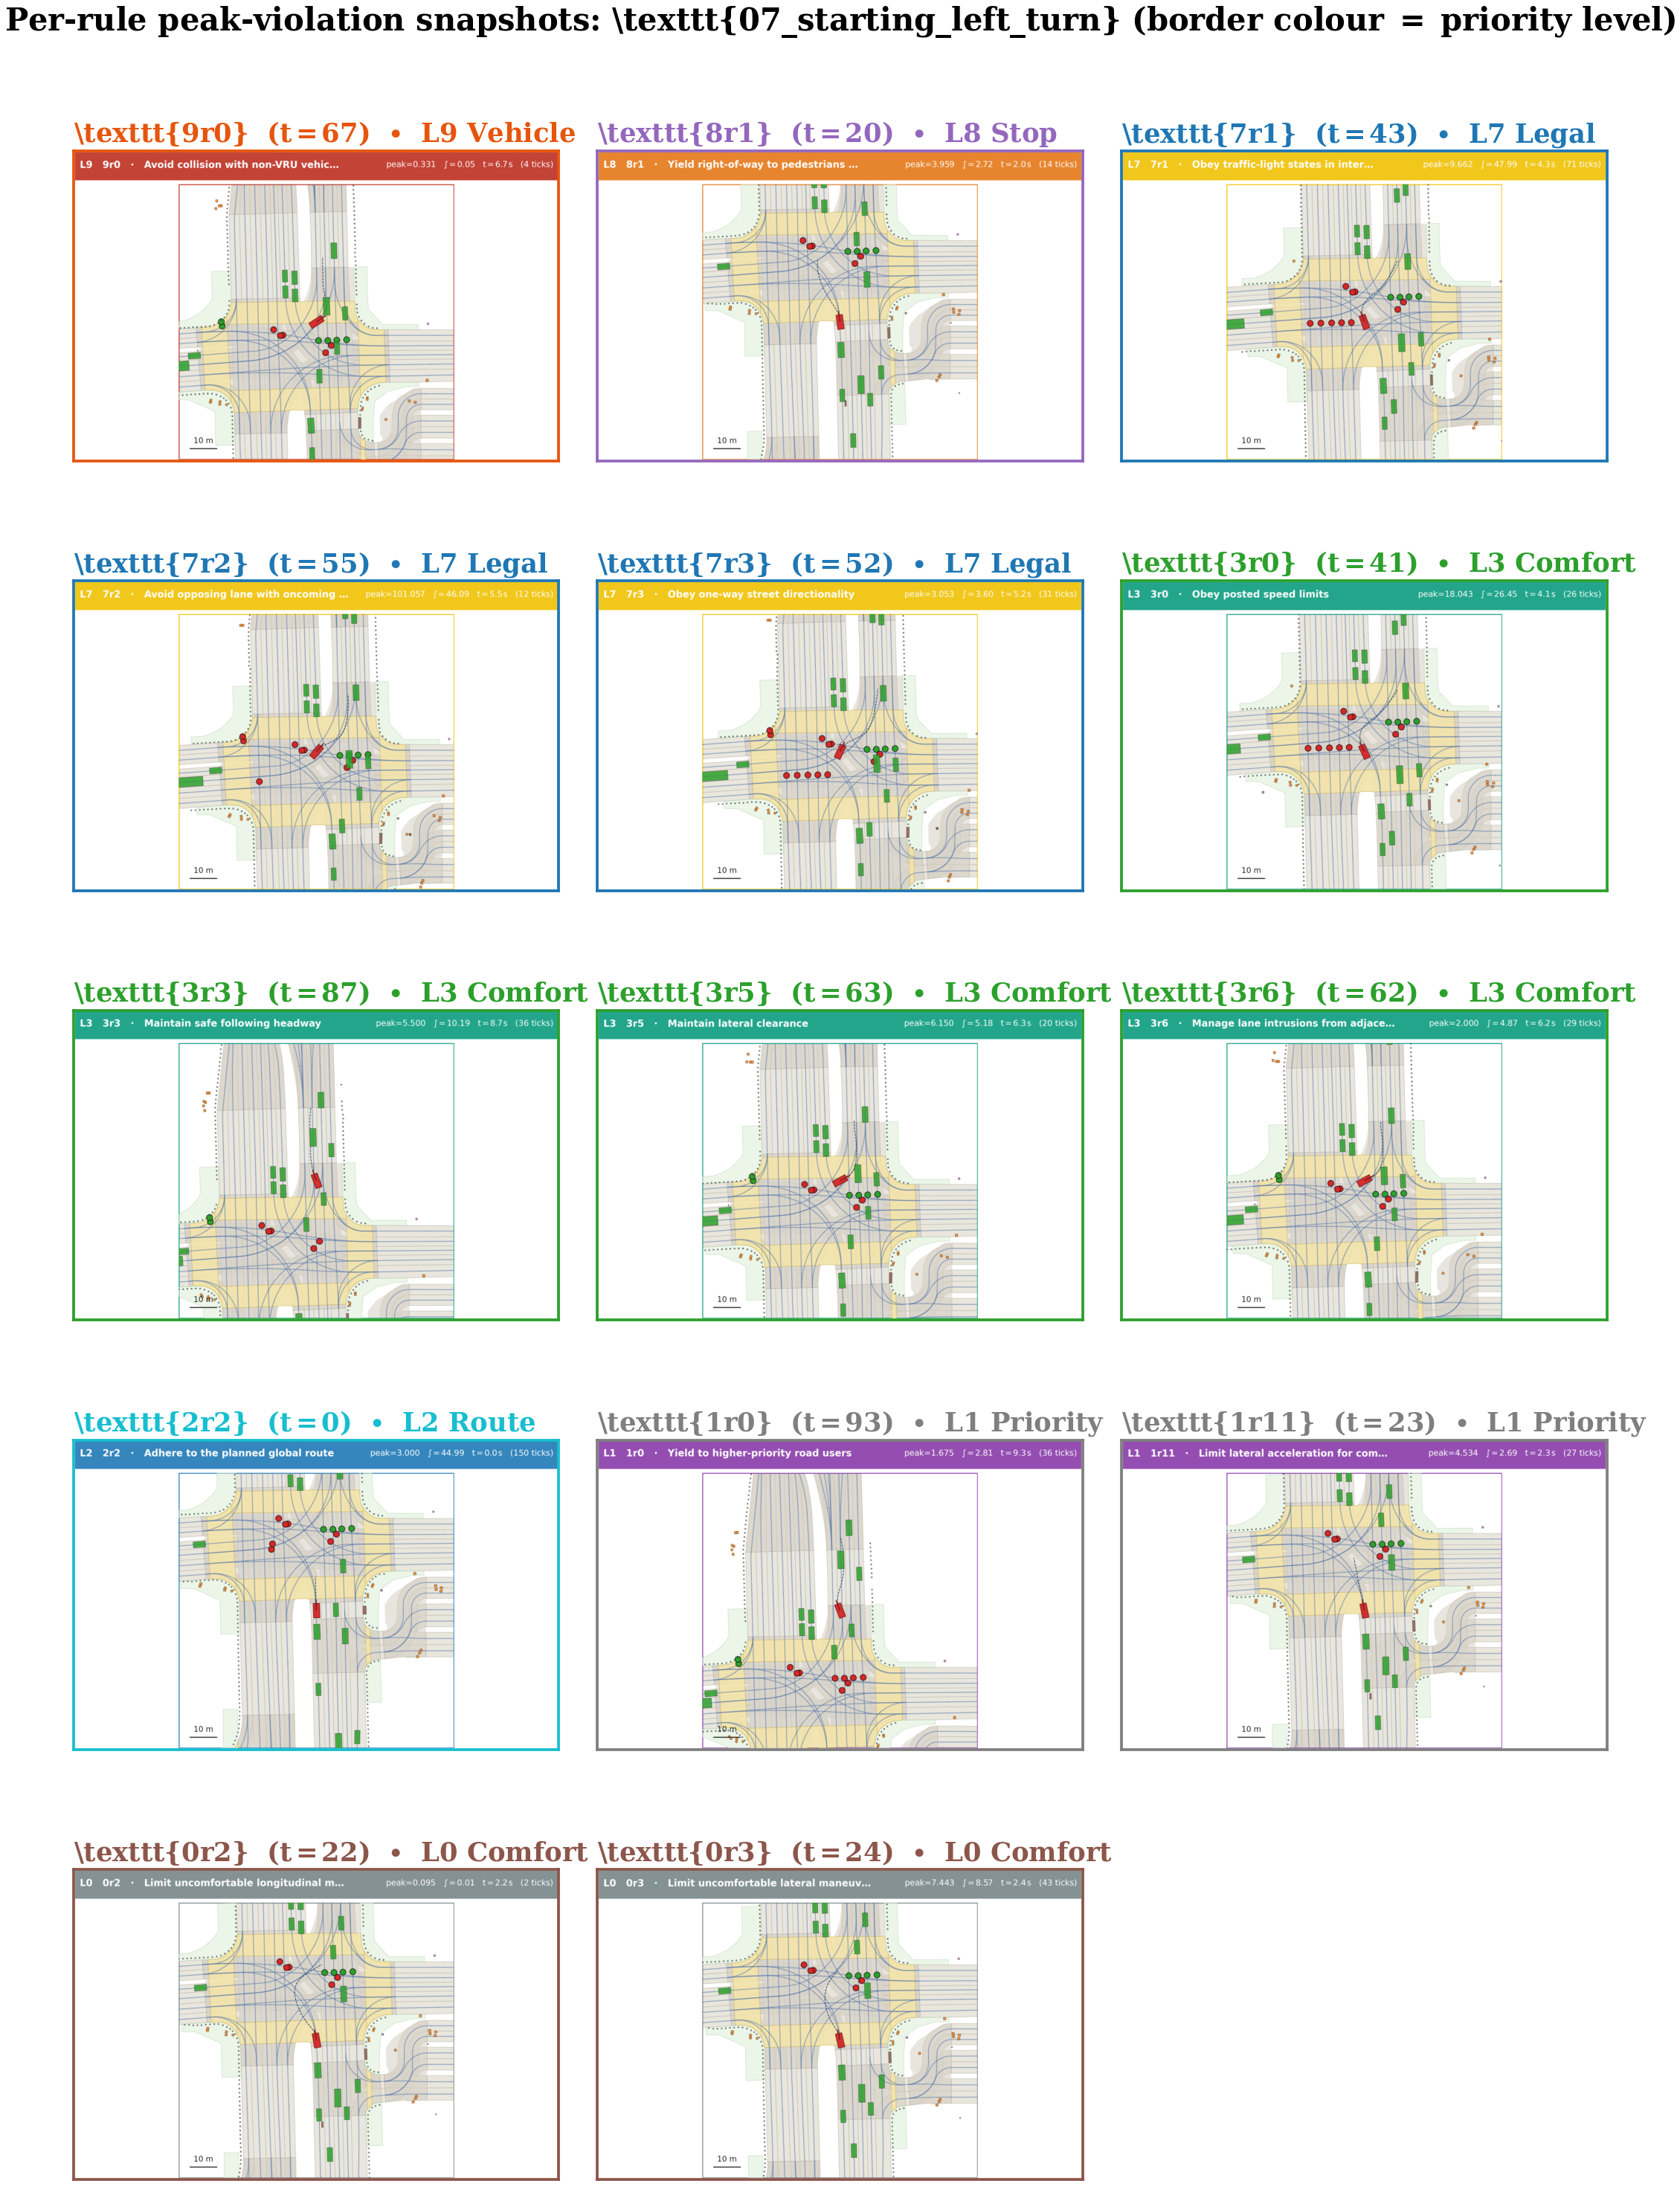
\includegraphics[width=\linewidth]{./Figures/fig14_violation_snapshots}
    \caption{Per-rule peak-violation snapshots for the representative scenario \texttt{07\_starting\_left\_turn} (3-column, 5-row grid, 14 tiles). Each tile is a map view of the ego, the agents, and the lane geometry at the tick of peak violation rate for the labelled rule. Tile-header colour encodes the priority level: $L_{10}$ VRU safety (red), $L_9$ vehicle safety (orange-red), $L_8$ stop / yield (purple), $L_7$ legal / lane (blue), $L_3$ comfort / headway (green), $L_2$ route adherence (teal), $L_1$ priority / yield (grey), $L_0$ longitudinal / lateral comfort (brown). Tiles are sorted by descending priority level. The complete gallery (143 per-rule snapshots + 16 per-scenario composites across the full 16-scenario benchmark) is in the online supplementary material.}
    \label{fig:violation_snapshots}
\end{figure}

Fig.~\ref{fig:violation_snapshots} provides representative qualitative evidence for the rule-by-rule violation profiles aggregated in Fig.~\ref{fig:a1_top_rule} and Fig.~\ref{fig:a3_rule_x_scenario}. Each snapshot captures the simulator state at the tick of peak violation rate for a specific rule. The snapshots serve a forensic role identical to that of the per-tick visualisation (Fig.~\ref{fig:qualitative_frame}) but indexed by rule rather than by scenario time. The complete gallery --- 143 per-rule snapshots plus 16 per-scenario galleries --- is released as supplementary material.
